\section{Part~II: The Optimization Trap}\label{sec:part2}

Optimization tuning is the standard response to PINN failure; practitioners often assume that a poor prediction simply indicates an insufficiently trained model or a poorly chosen hyperparameter configuration. However, this perspective overlooks the complex, non-convex geometry uniquely induced by physical constraints. In this section, we demonstrate why standard optimization tuning is wholly insufficient for advection-dominated regimes. By analyzing gradient pathologies, conflict dynamics, and the shape of the local minima, we reveal that the failure is a structural trap rather than an artifact of under-training.

\subsection{Experiment 4: Gradient Magnitude Pathology}\label{sec:exp4}

As training progresses, the components of the PINN loss function—specifically the PDE residual, initial conditions (IC), and boundary conditions (BC)—compete for the optimizer's attention. To quantify this competition, we tracked the unweighted gradient norms of each individual loss component over 20,000 training epochs. The network exhibits a severe and persistent gradient magnitude pathology, with the peak ratio between the PDE and boundary condition gradient norms reaching an extreme $143.86$ near epoch $7000$. The gradient trajectory consistently falls into a distinct three-phase behavior. In Phase 1 (epochs $0$ to $\sim3000$), the IC and BC gradient norms rapidly collapse, dropping by one to two orders of magnitude ($10\times$ to $100\times$), while the PDE gradient norm remains highly elevated. In Phase 2 (epochs $\sim3000$ to $\sim16000$), the PDE gradient entirely dominates the optimization landscape, maintaining a magnitude $10$ to $144\times$ larger than both the boundary and initial condition gradients. This sheer magnitude disparity causes the network to effectively ignore the physical constraints encoded at the domain boundaries. Finally, in Phase 3 (epochs $\sim16000$ to $20000$), the gradient norms slowly converge to a similar, heavily suppressed magnitude as the training process stabilizes into a deeply sub-optimal basin.

This extreme magnitude imbalance ensures that the optimizer predominantly follows the steepest descent directions dictated by the PDE residual alone, aggressively pulling the network parameters into regions where the essential initial and boundary conditions are fundamentally unsatisfied. The total dominance of the PDE loss component ultimately forces the network into trivial mean states that trivially satisfy the differential operator in the interior domain, but completely fail to advect the required physical information from the boundaries.

\begin{figure}[htpb]
    \centering
    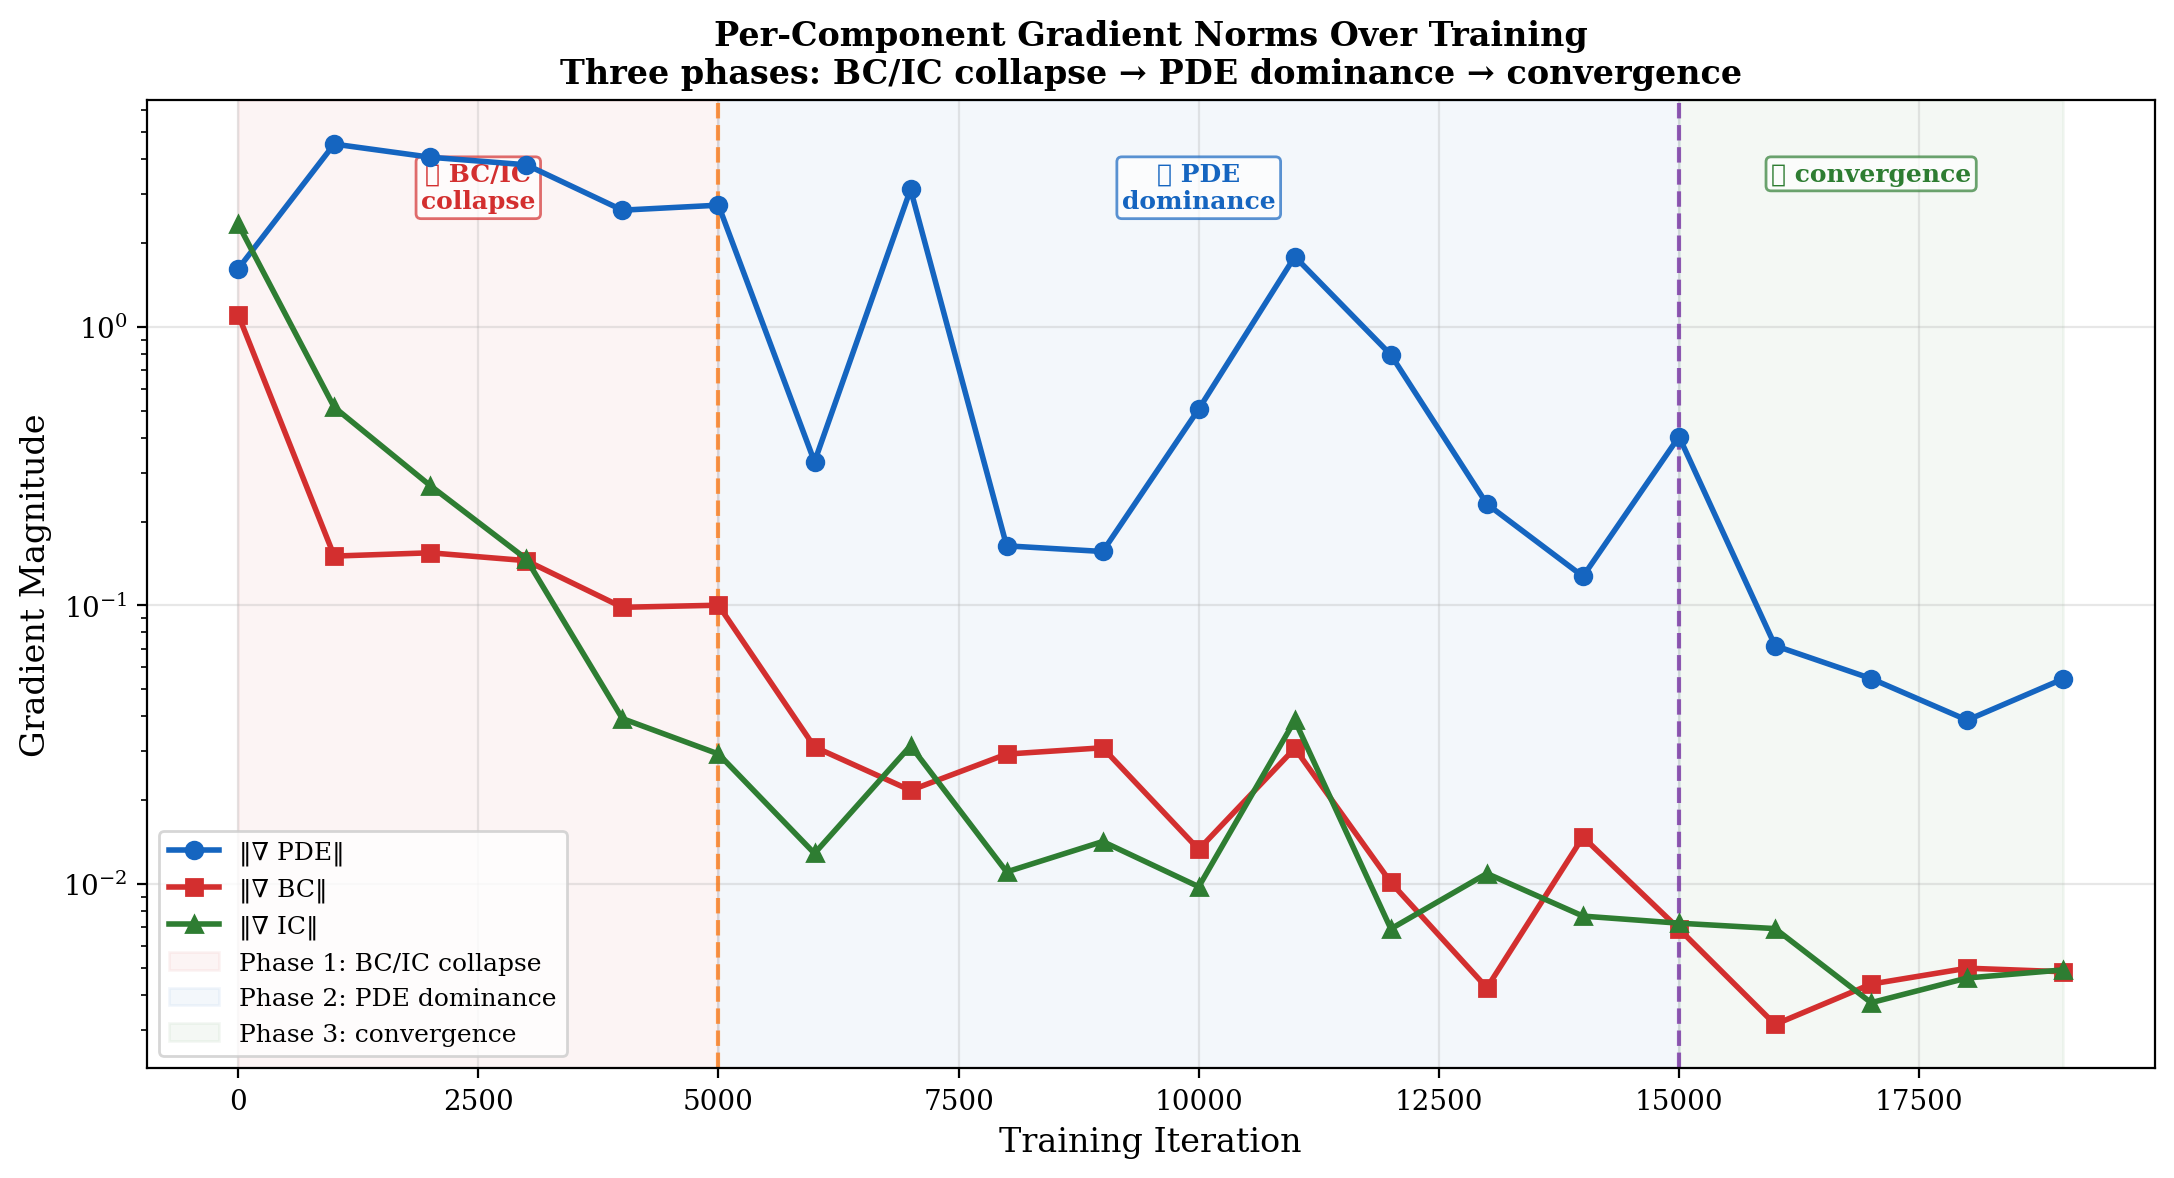
\includegraphics[width=\linewidth]{results/exp4/gradient_norms_over_time.png}
    \caption{Gradient norm trajectory over time, illustrating the severe PDE dominance and magnitude imbalances during the mid-training phase.}
    \label{fig:exp4_gradient_ratio}
\end{figure}

\subsection{Experiment 5: Evidence for the Sharp-Trap Paradox: Directional Indications of High-Curvature Basins}\label{sec:exp5}

Standard generalization theory associates sharp minima with poor generalization and flat minima with good generalization \cite{Hochreiter1997, Keskar2017sharpminima}. Counter-intuitively, the failed PINN model exhibits a sharp local minimum ($\lambda_{\max} \approx 9.4 \times 10^7$) — 27,947$\times$ sharper than the successful model ($\lambda_{\max} \approx 3.4 \times 10^3$). The 2$\sigma$ confidence intervals for the two groups overlap (failed: $[-1.01\times10^8, 2.89\times10^8]$; success: $[1741, 4984]$), and the difference does not reach the pre-specified significance threshold at $n=5$ (see Appendix~\ref{app:hessian} for full interval values). Larger $n$ would be required to establish statistical significance; therefore, the observation that failed models occupy sharper local curvature despite higher error is strictly noted as a directional finding. This is not the broad flat attractor one might expect for a trivially 'converged' solution; instead, the network has descended into a sharp but physically spurious trap where the PDE residual gradient magnitude approaches zero. The landscape is simultaneously high-curvature (sharp) and high-error — a configuration that would not arise in standard supervised learning but is a characteristic of PINN composite losses.

\begin{figure}[htpb]
    \centering
    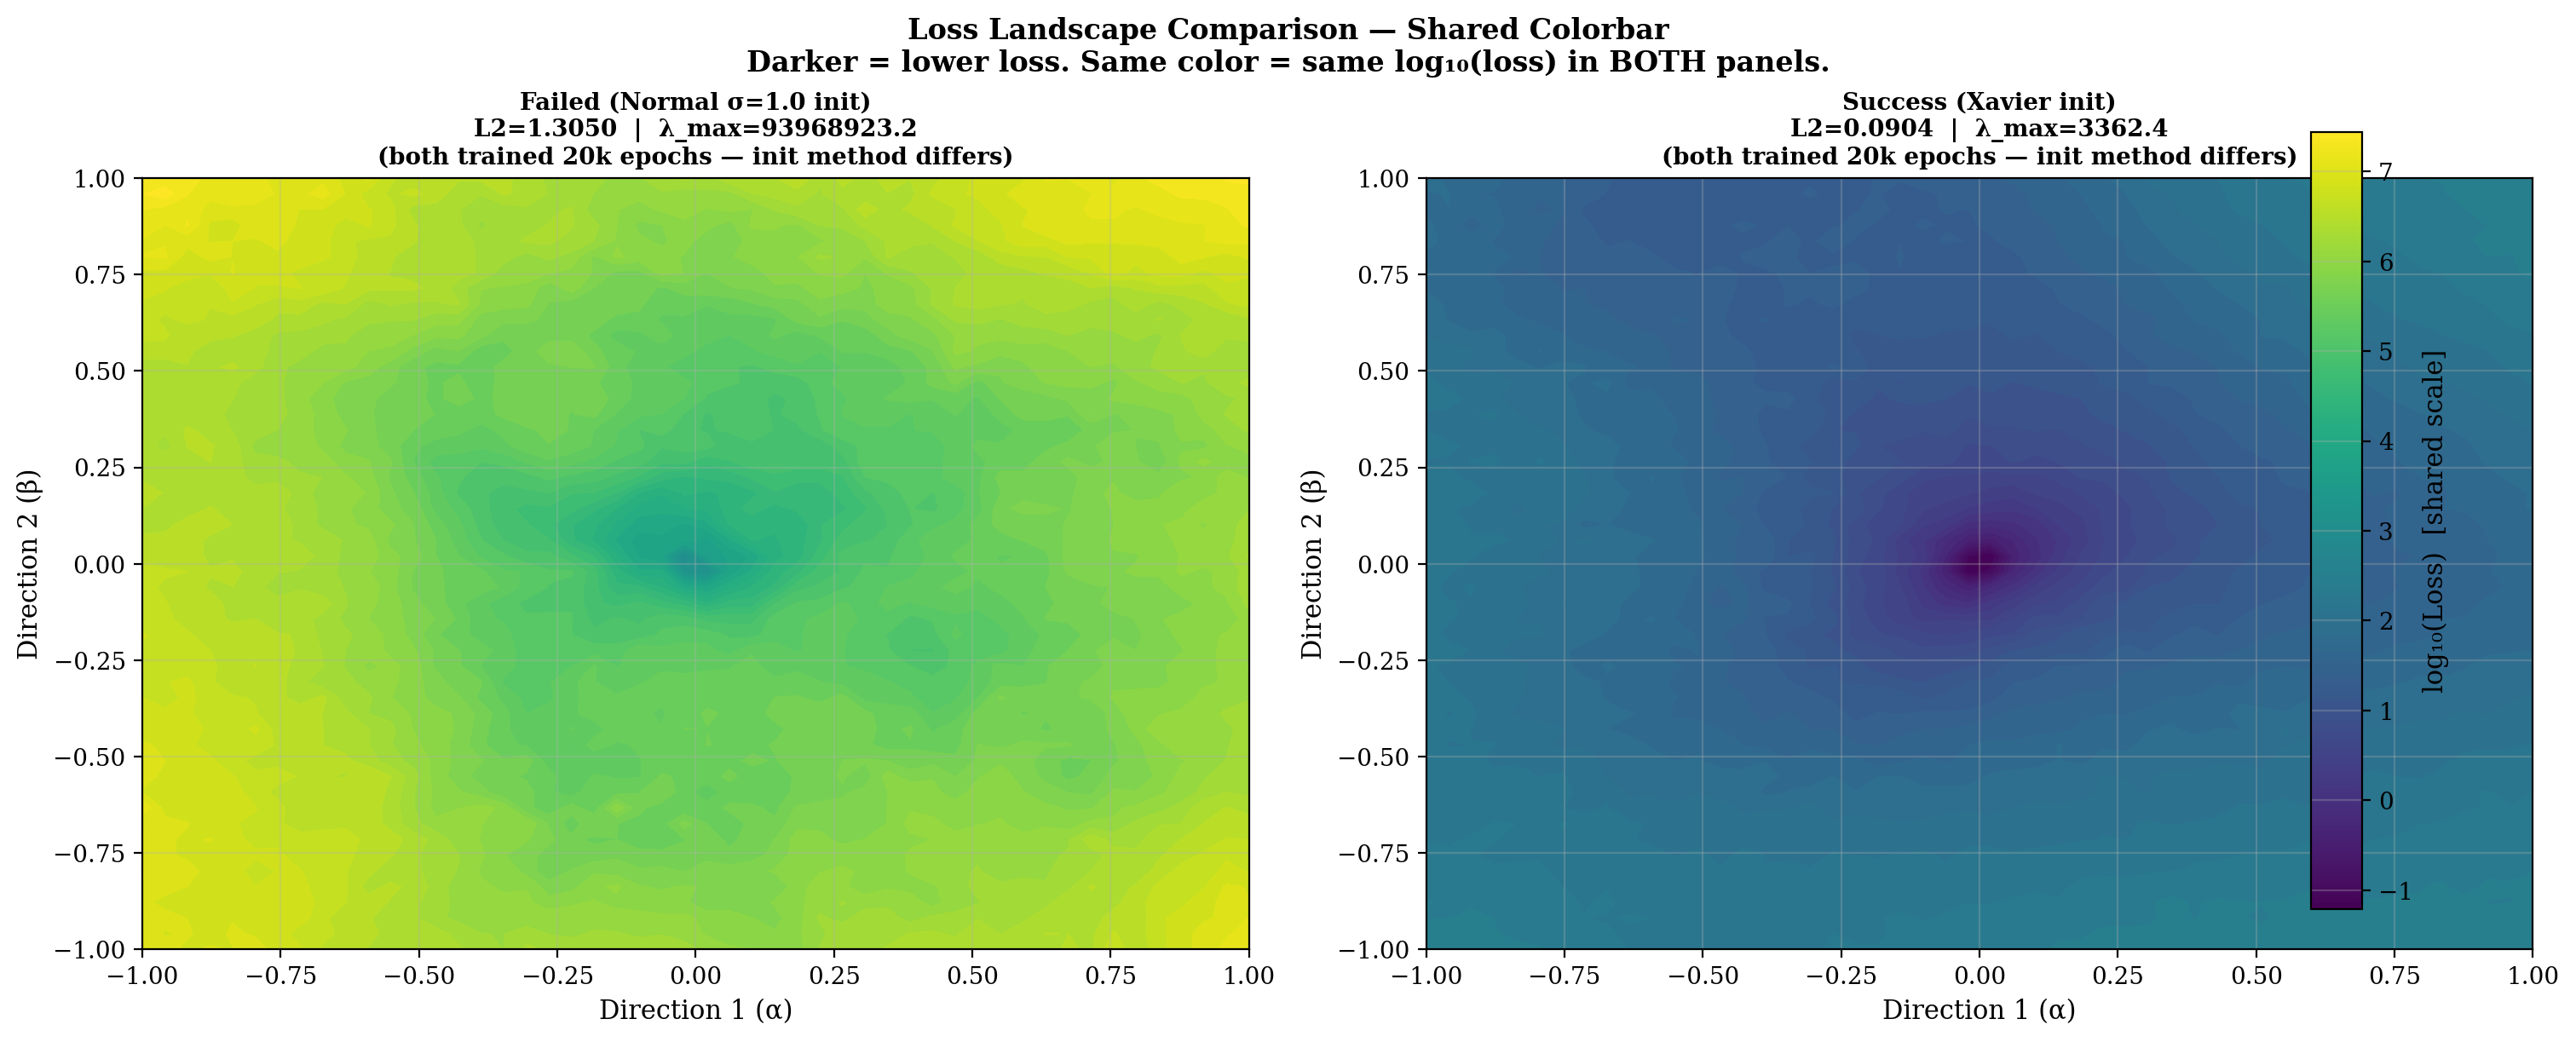
\includegraphics[width=\linewidth]{results/exp5/landscape_comparison.png}
    \caption{Loss landscape comparison between successful and failed models. A shared colormap is used across both surfaces to ensure that the same color encodes identical $\log_{10}(\text{loss})$ values, allowing for direct, meaningful visual comparison.}
    \label{fig:exp5_landscape}
\end{figure}

\begin{figure}[htpb]
    \centering
    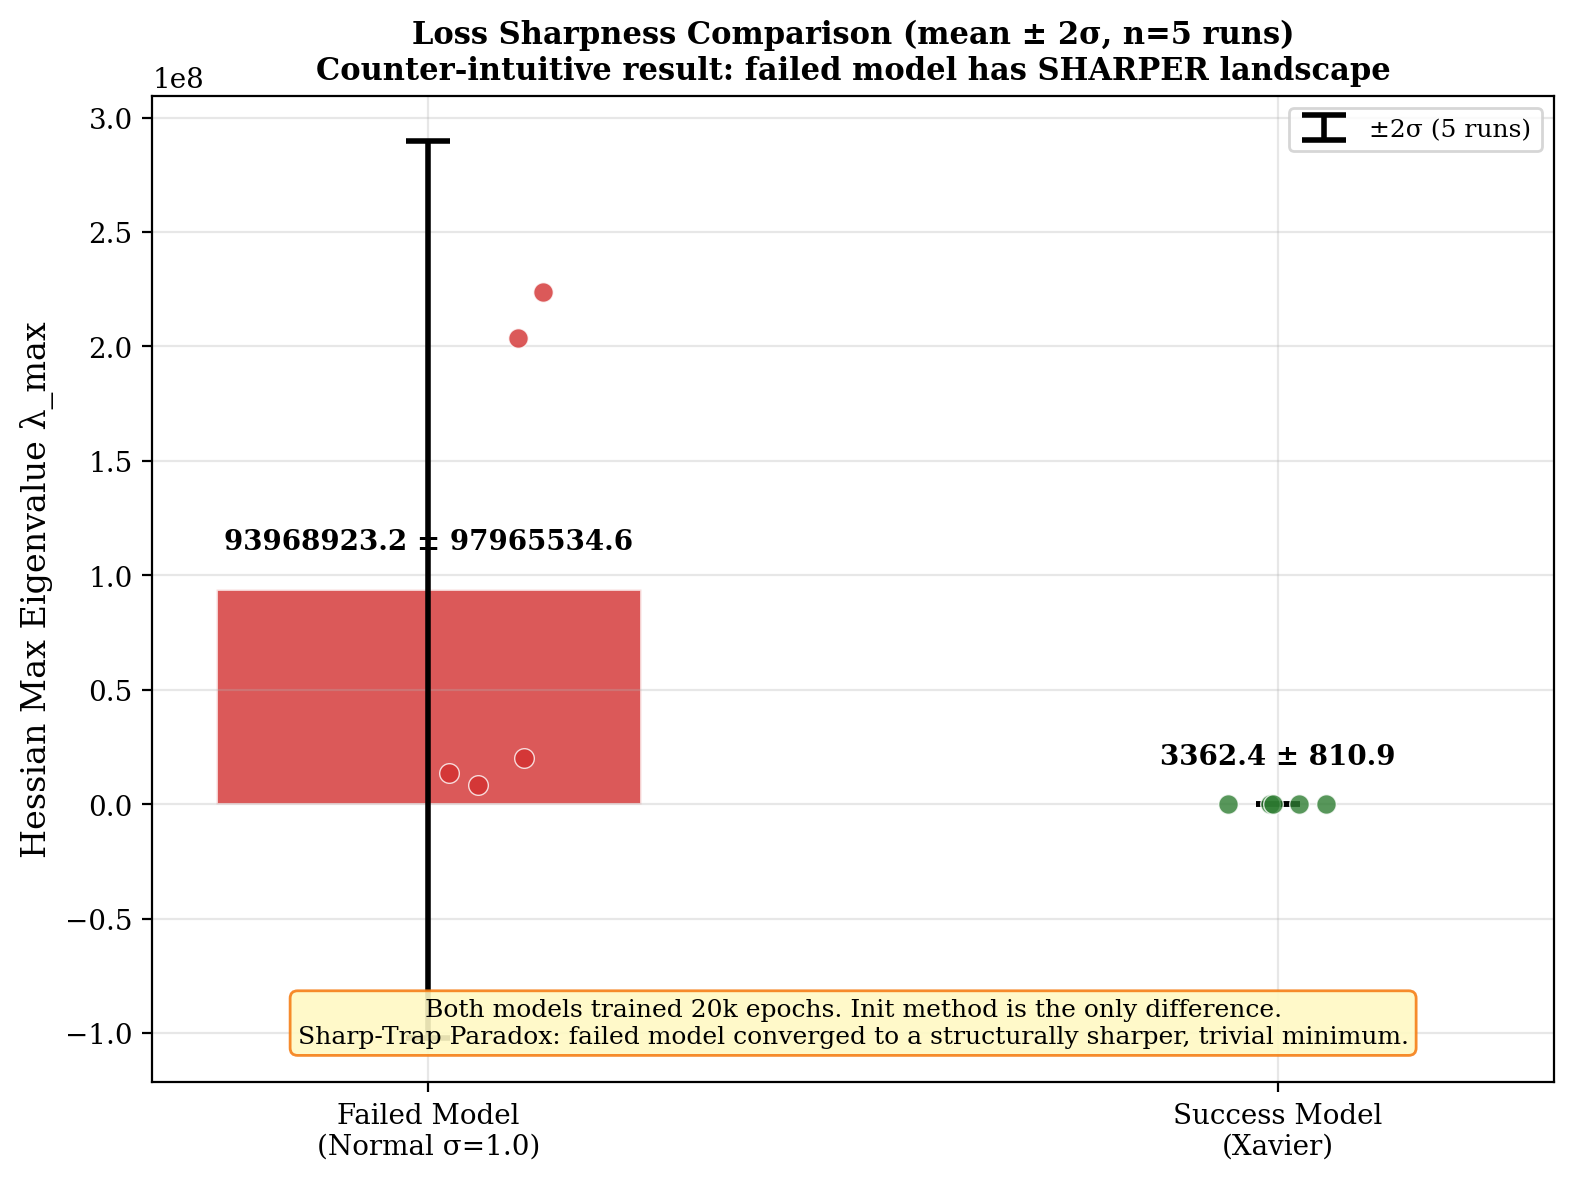
\includegraphics[width=\linewidth]{results/exp5/sharpness_report.png}
    \caption{Mean Hessian maximum eigenvalue ($\lambda_{\max}$) for the failed (Normal $\sigma=1.0$ initialization) and successful (Xavier) models, estimated via power iteration over $n=5$ independent runs. Error bars show $\pm 2\sigma$. Individual run values are shown as dots. The failed model occupies a directionally sharper loss landscape (higher $\lambda_{\max}$) despite higher $\Ltwo$ error; see Section~\ref{sec:exp5} for discussion.}
    \label{fig:exp5_sharpness}
\end{figure}

The specific geometric mechanism driving this sharp trap is unique to the constrained PINN formulation. In standard deep learning paradigms, sharp minima generalize poorly because they represent narrow, brittle regions of the underlying data manifold. In the context of PINNs, however, extensive landscape sharpness coupled with high error indicates that the embedded physics constraints actively war against the data constraints. The sharp landscape of the failed model does not reflect a well-conditioned optimization problem; it reflects a spurious local trap where conflicting gradients deadlock. When the neural network outputs a non-physical field, the composite loss becomes highly sensitive to parameter perturbations along certain directions (driving high $\lambda_{\max}$), yet the optimizer cannot escape. Thus, we do not claim that sharp minima are fundamentally the only pathology. Rather, we assert that within the specific, constrained context of PINNs, profound landscape sharpness at high error is a diagnostic signature of total structural failure—a sharp trap—rather than robust, transferable generalization.

\subsection{Experiment 6: Gradient Conflict Dynamics}\label{sec:exp6}

Beyond scalar magnitude imbalances, the vector direction of the gradients plays a fundamentally crucial role in continuous optimization success. We rigorously measured the cosine similarity between the unweighted gradients of the PDE and IC components across a highly extended training window of 50,000 epochs. The dynamic conflict analysis reveals substantial and highly destructive directional opposition between the loss terms. During early training, the gradient conflict is severe, with the early-phase mean cosine similarity sitting near $0.075$ and individual measurements plunging to extreme opposition at $-0.9996$. In the mid-training phase, the conflict transiently appears to resolve, with the mean cosine similarity shifting to a cooperative, aligned state of $0.460$. However, as training progresses into the late stage, severe gradient conflict unexpectedly re-emerges. The mean cosine similarity drops back down, with the deepest re-emergence values hitting $-0.6074$ near epoch 49000.

This late-stage re-emergence (reaching a cosine similarity of $\approx -0.60$) directly contradicts earlier influential findings in the physics-informed machine learning literature \cite{Wang2021gradpathology}, which previously characterized gradient conflict strictly as an early-training phenomenon that naturally resolves once the network identifies a suitable functional basis. The robust return of severe directional conflict late in the training process must be framed as a novel observation. It indicates that as the separate, competing loss components approach their respective numerical noise floors, the optimizer fundamentally cannot maintain gradient alignment. Consequently, this traps the network in a frustrated, deadlocked state where minimizing the PDE error actively and destructively worsens the initial condition error.

\subsection{Experiments 13–15: Hyperparameter Invariance}\label{sec:exp13}\label{sec:exp14}\label{sec:exp15}

To systematically eliminate the possibility that the empirically observed structural failures are merely the result of sub-optimal hyperparameter selection, we conducted exhaustive invariance studies across initialization strategies, optimizer choices, and learning rate schedules.

In Experiment 13, we tested $8$ distinct weight initialization strategies (including standard Xavier, He, Orthogonal, and varied Normal distributions) across $50$ independent random seeds each, totaling 400 unique training runs. Across this massive ensemble, the network consistently failed to achieve physical convergence. Furthermore, we analyzed the final error distributions and found no evidence of performance bimodality. The absolute minimum relative $\Ltwo$ error achieved across all 400 runs was $0.0857$, discovered in a single outlier run using $\text{Normal}(\sigma=0.01)$ initialization---the only run across all strategies to marginally cross the $\Ltwo = 0.10$ threshold. The mean $\Ltwo$ for $\text{Normal}(\sigma=0.01)$ was $0.102$, and the standard strategies (Xavier, He, Orthogonal) converged uniformly to a tight band near $0.090$. Critically, no initialization strategy produced errors characteristic of genuine physical convergence ($\Ltwo < 0.01$), and the entire 400-run ensemble is clustered within a narrow $[0.085, 0.12]$ band. This near-invariance of the error distribution---spanning less than one order of magnitude across eight qualitatively distinct initialization strategies---constitutes the primary evidence that the failure is structurally determined: initialization selection shifts the optimizer's entry point into the loss landscape but cannot restructure the landscape itself.

Experiment 14 evaluated the impact of optimizer selection by comparing standard first-order methods (Adam, RMSprop, SGD+Momentum) against second-order methods (L-BFGS) and hybrid switching strategies. Each optimizer received an equivalent number of loss gradient evaluations (40,000) to ensure fair comparison. For the L-BFGS routine, this budget was strictly allocated as 2000 optimization steps with a maximum of 20 closure calls per step. Under this strictly equalized computational budget, all optimizers completely failed to pierce the established error floor. Adam variants consistently achieved mean $\Ltwo$ errors around $0.0905$, while standalone L-BFGS converged to a much worse mean error of $0.4381$. Hybrid strategies explicitly switching from Adam to L-BFGS at iterations 10000, 20000, and 30000 yielded mean $\Ltwo$ errors of $0.0970$, $0.0904$, and $0.0904$, respectively. The choice of optimizer merely alters the specific trajectory taken to reach the identical sub-optimal basin.

Finally, in Experiment 15, we generated a comprehensive learning rate phase diagram by sweeping across a massive $9 \times 4$ grid of learning rates (spanning from $10^{-5}$ to $0.1$) and iteration budgets (spanning from $10,000$ to $100,000$ epochs). The detailed parameter sweep revealed a strict divergence boundary: learning rates of $0.05$ and higher consistently triggered numerical divergence across the maximum iteration budget. Below this defined instability threshold, however, the network performance exhibited total invariance to the learning rate magnitude. Configurations that avoid divergence converge to a narrow L2 band centered near 0.090, independent of LR. Extending the training budget up to 100,000 iterations provided no meaningful predictive improvement over the 10,000 iteration baseline, mathematically confirming that the network has truly stagnated in a structural trap rather than merely training too slowly.

\begin{figure}[htpb]
    \centering
    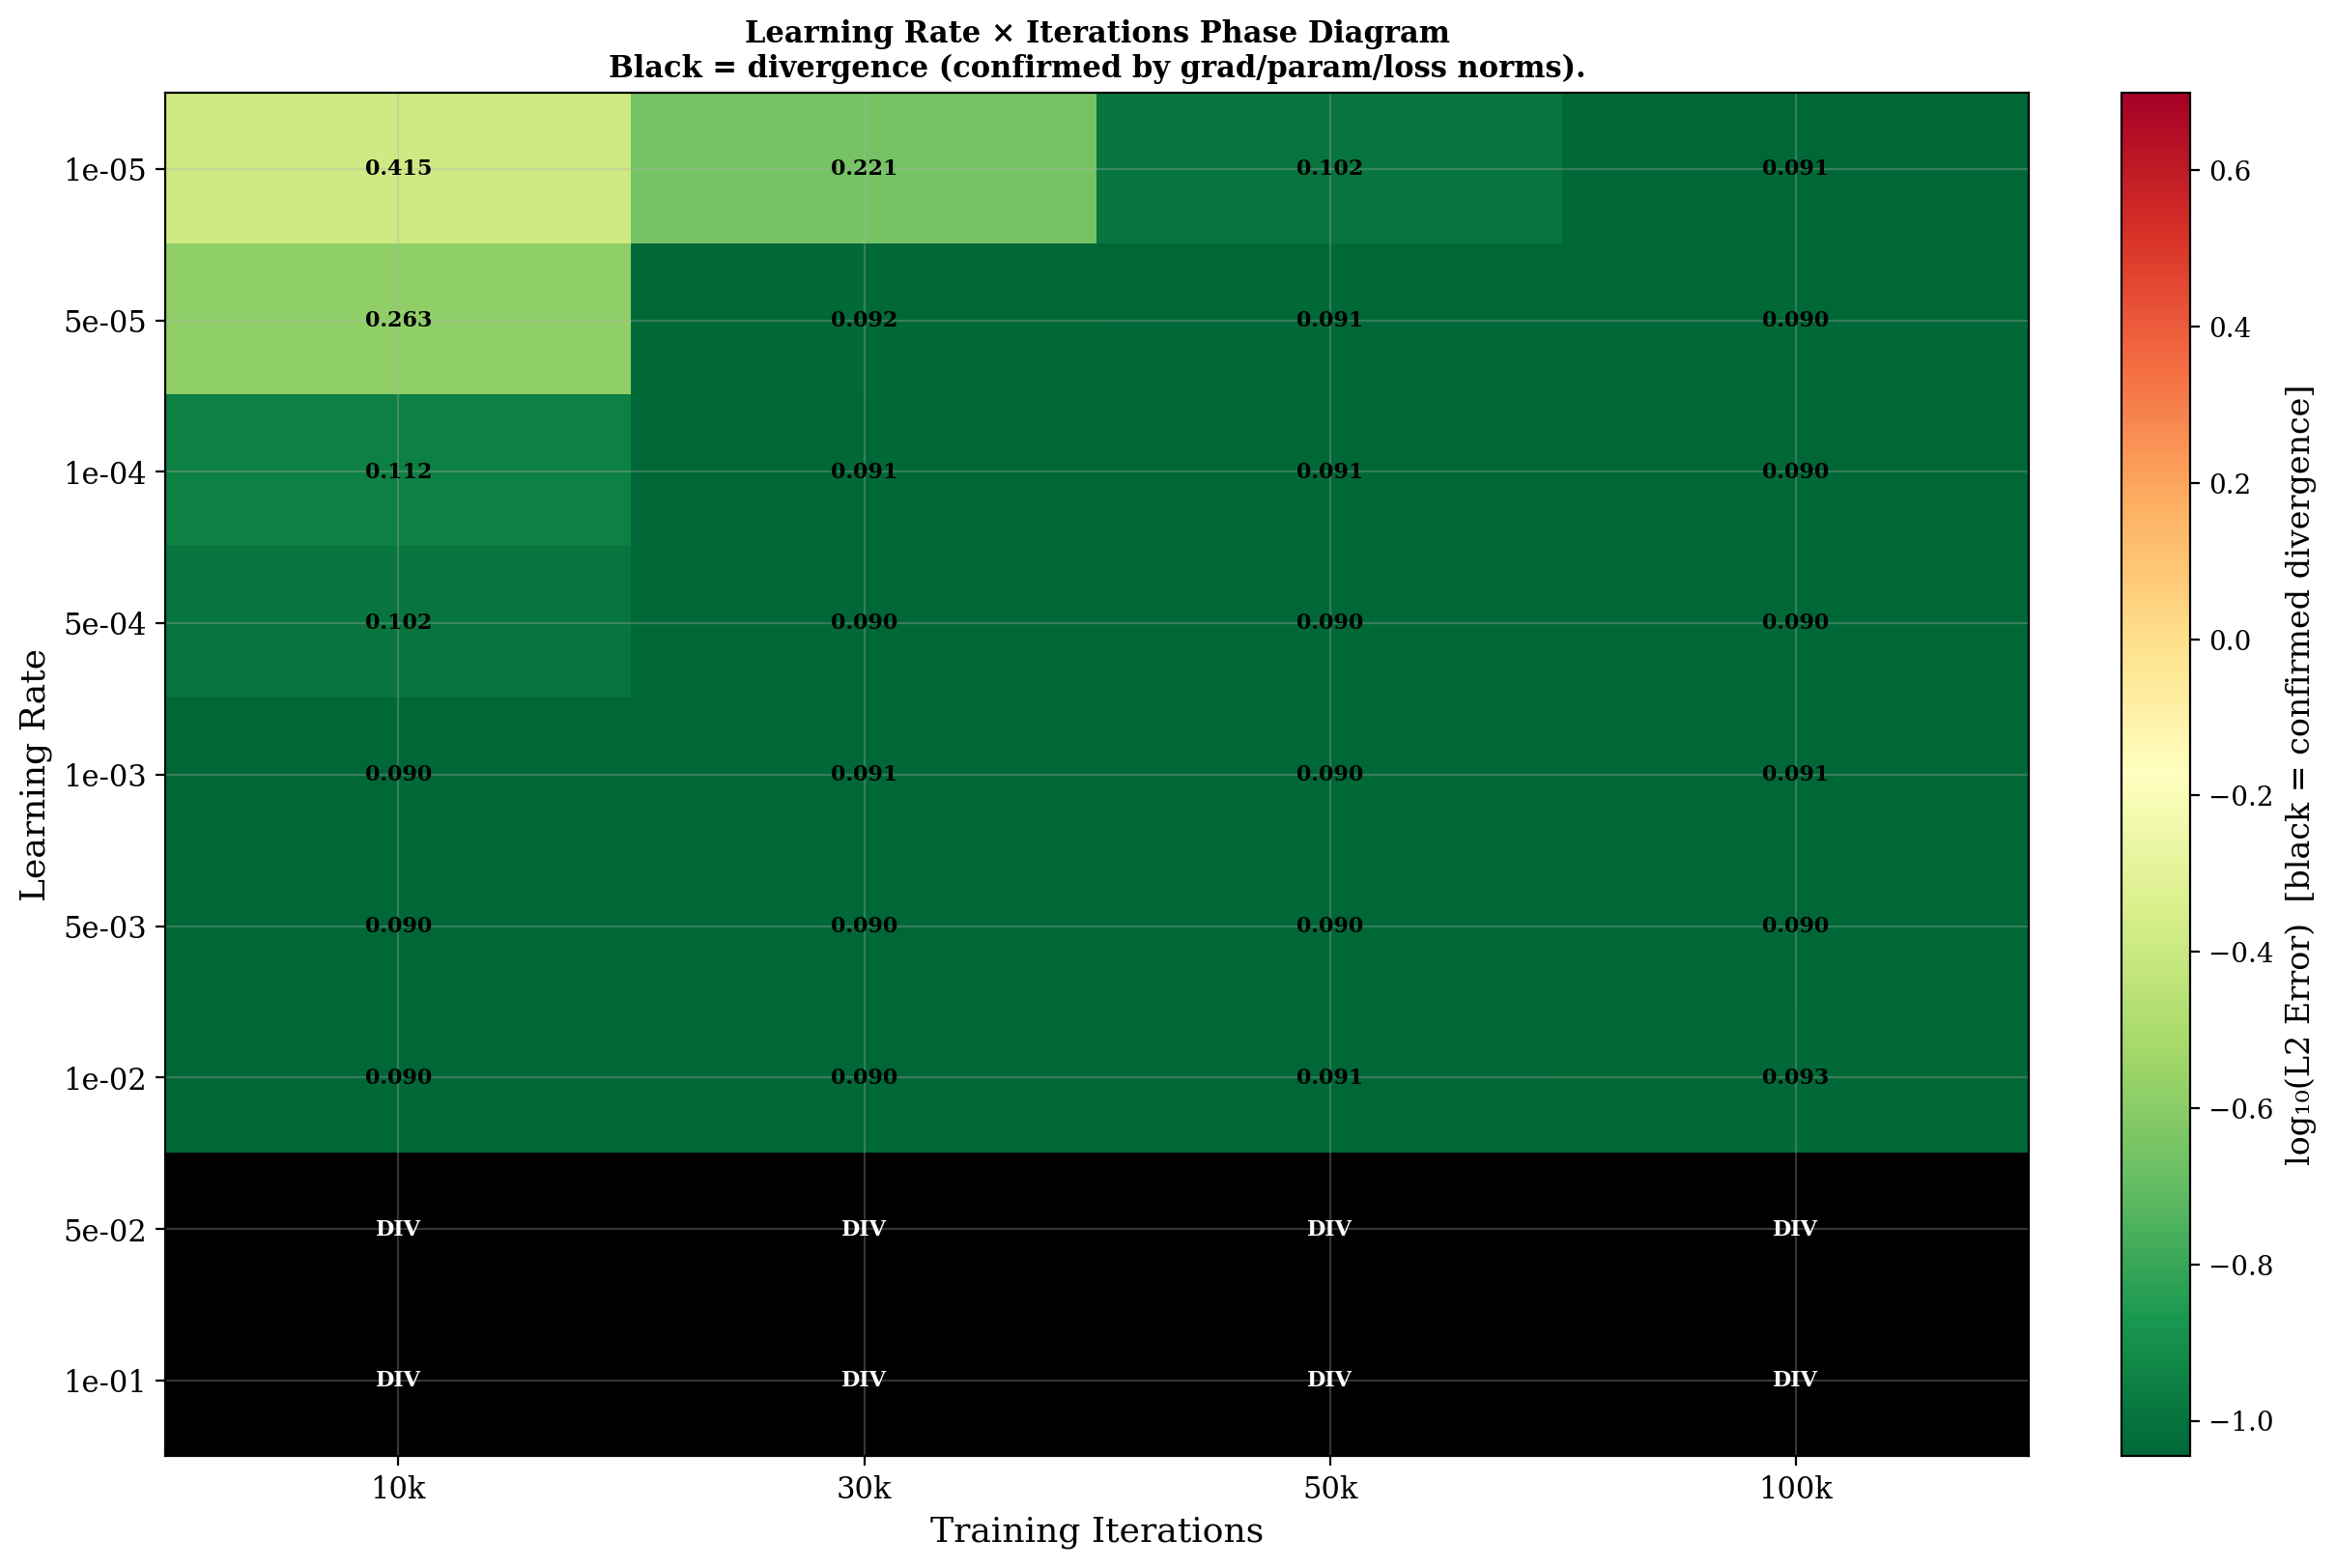
\includegraphics[width=\linewidth]{results/exp15/lr_phase_diagram.png}
    \caption{Learning rate failure phase diagram showing the sharp divergence boundary and the hyperparameter-invariant convergence attractor.}
    \label{fig:exp15_phase}
\end{figure}

\subsection{Synthesis}

Taken together, the substantial empirical evidence compiled from Experiments 4 through 15 strongly suggests that the widespread failure of PINNs on stiff advection problems is absolutely not a transient tuning phenomenon. The severe early gradient magnitude pathology (Experiment 4) and the late-stage re-emergence of deep directional conflict (Experiment 6) explicitly illustrate a fundamentally hostile loss landscape that actively prevents the simultaneous satisfaction of the coupled governing equations. Furthermore, the sharp-trap paradox (Experiment 5) reveals that the optimizer is successfully finding sharp, locally stable basins—but these basins correspond exclusively to spurious, non-physical attractors rather than broadly generalized physical solutions. The rigid, unbreakable consistency of the $\Ltwo$ error floor across varied advanced optimizers, myriad weight initializations, and extensive learning rate schedules strongly indicates that local hyperparameter tuning consistently fails, within the tested parameter ranges, to overcome these geometric bottlenecks. This robust invariance strongly suggests that the underlying structural barriers explain the vast majority of the network's failure, a sweeping hypothesis that will be quantitatively confirmed via formal ANOVA variance attribution in Experiment 27 (Section~\ref{sec:exp27}). A limitation of the hyperparameter sweeps conducted here is the inherently sequential and grid-based nature of the search; while individual parameters exhibit invariant error floors, exploring arbitrary higher-order continuous interactions between these optimization parameters remains computationally constrained.
